\documentclass[main.tex]{subfiles}
\begin{document}

We explored a solution for a person to become a good behaving driver. We introduced an intelligent device called SEDA which easily fitted into a driver eye wear, glasses or head gear. Instead of monitoring for enforcement, the SEDA design goal was a human-centred design and encouraged user participation. The SEDA was designed for a Ubiquitous Computing device and for a personal gadget use. It was self-situation-awareness system for a user such that it did focus on their own safety while on the road. We embraced safer future by how we transferred a good driving behaviour to our future generation. We further presented that the system comprise of distributed computing components such as the SEDA base mobile app to configure the device and SEDA backend cloud service for intelligence processing. The overall system architecture aimed to harness the power of Machine Learning techniques to classify the data acquired from the SEDA and train the classification model on a driver behaviour to produce a safer driving profile. This profile were then loaded onto the SEDA device and gave advice based on the difference between the loaded profile and the actual active decision making of a driver.
\\

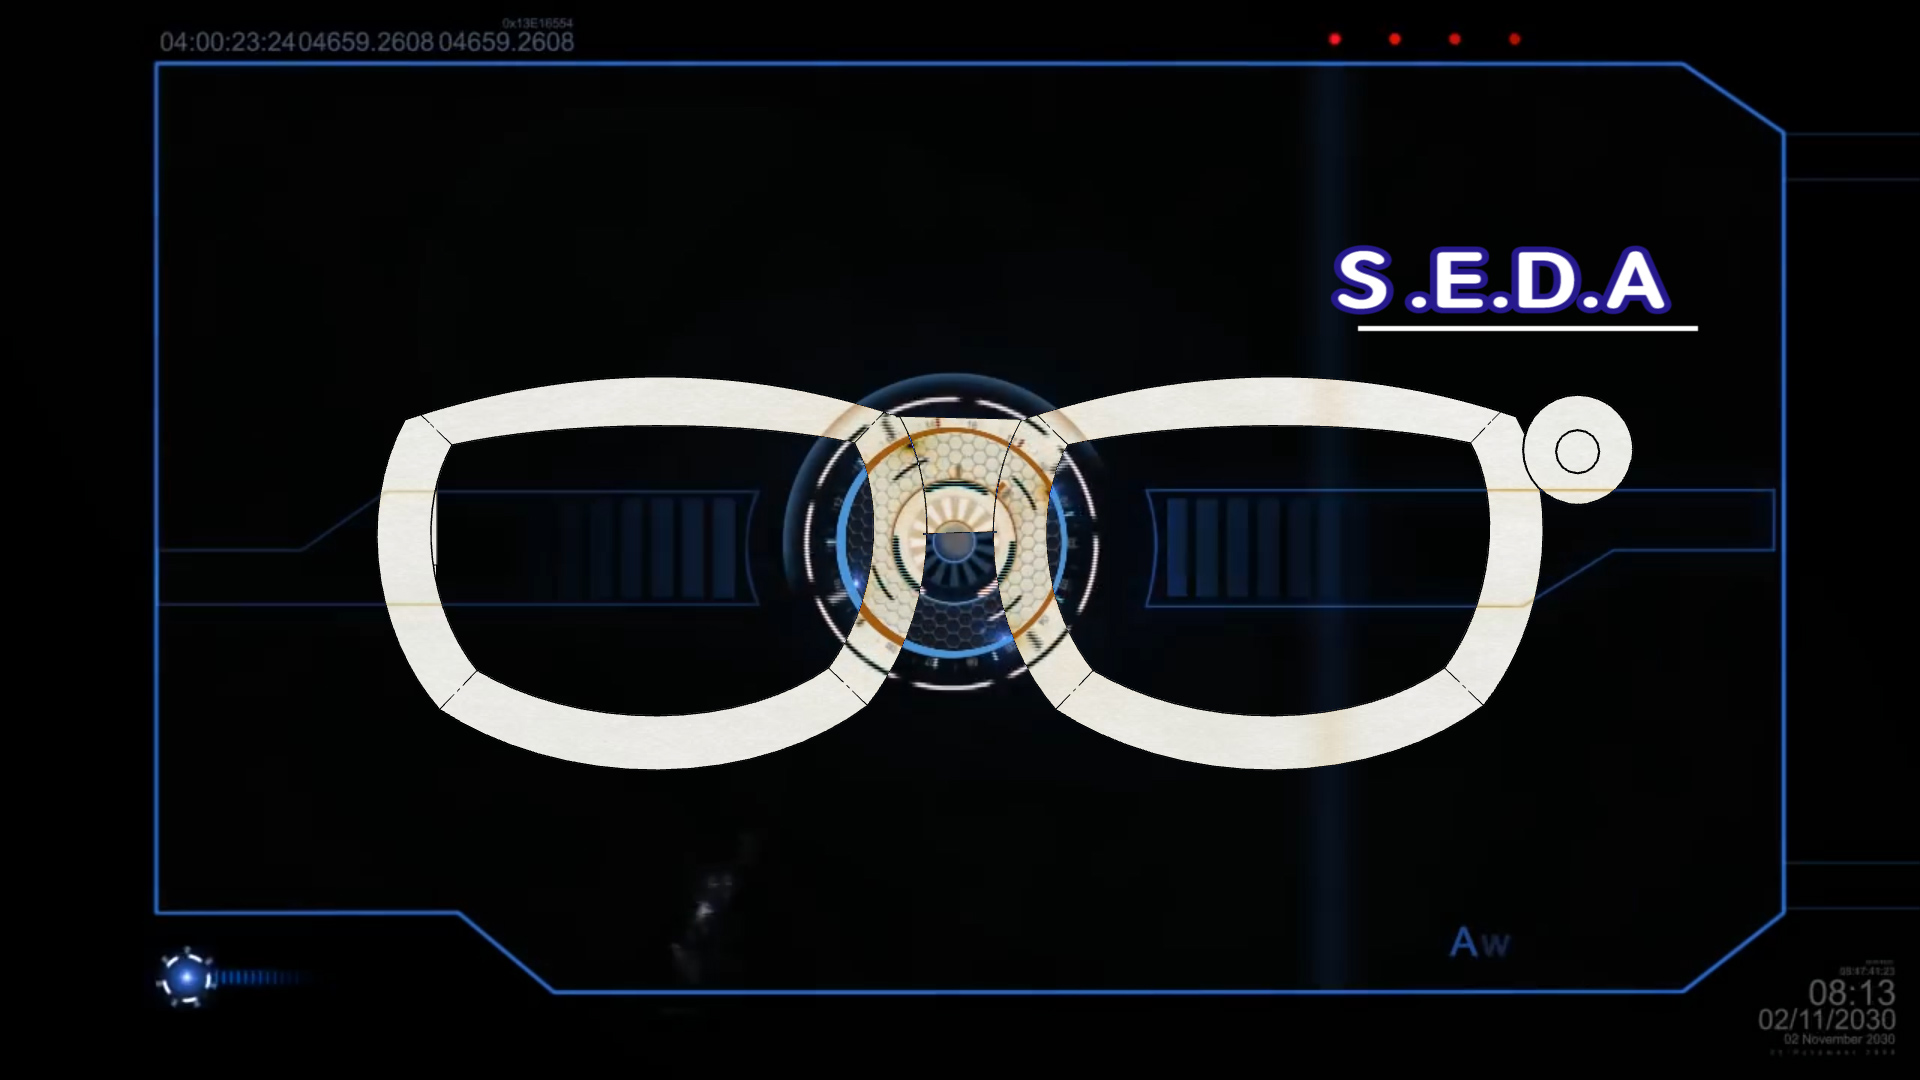
\includegraphics[width=\columnwidth]{seda_concept}

\end{document}